\section{Motivation}

\subsection{History Signals Do Not Encode Death Cohorts}

History-based placement asks: what did this block look like before?  \dogi-style policies observe LBA, previous LBA, access interval, segment frequency, and prior placement state.  These features are meaningful for ordinary payload updates because they capture hotness and locality.  A post-quantum secret asks a different question: which objects will die together when the protocol state advances?  The answer requires at least intent and epoch.

This distinction creates two failure modes.  The first is semantic: the baseline leaves expired secret blocks in zones that are not safely resettable because the zone also contains payload or long-lived metadata.  The second is performance: under sufficient free-zone pressure, mixed death cohorts force valid-block migration and raise WAF.  The first failure can appear even when WAF is near 1.0; the second appears only in harder pressure workloads.

\begin{figure}[!t]
\centering

\includegraphics[width=0.62\columnwidth]{../artifacts/figures/fast-style/fig2-motivation-semantic-gap-legend.pdf}\\[-0.4em]
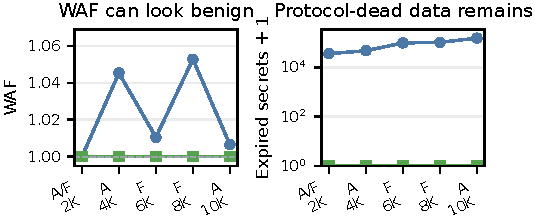
\includegraphics[width=0.98\columnwidth]{../artifacts/figures/fast-style/fig2-motivation-semantic-gap.pdf}
\caption{Motivation diagnostic: WAF is not enough to expose the PQC failure mode.  \dogi-style placement can look benign on storage-visible WAF while still stranding expired PQC secrets; \system-\dogi keeps payload on history placement but routes lifecycle objects by death cohort.}
\label{fig:motivation-semantic-gap}
\end{figure}

Figure~\ref{fig:motivation-semantic-gap} shows the diagnostic reason this paper does not use WAF alone as the motivation.  On DOGI-compatible YCSB carriers, \dogi-style placement often keeps physical WAF close to 1.0 because the payload locality signal is still useful.  At the same time, expired PQC secrets remain stranded because the storage-visible history does not encode epoch close.  \system-\dogi removes those protocol-dead secrets.  It routes only lifecycle objects through the death-cohort path.

\subsection{Easy Workloads Are Not Enough}

A clean PQC-only epoch trace makes \system look too good and is not a fair test of \dogi.  Our evaluation therefore treats such traces as sanity checks only.  The hard tests keep DOGI's normal locality signals and then add realistic PQC lifecycle writes.  Concretely, the workload matrix contains: DOGI-style six-axis fairness, YCSB-A/F pressure, FAST-style Sysbench pressure, dynamic service pressure, and QUASAR-hostile robustness.

\subsection{The Upper Bound Gives Design Requirements}

DOGI uses NoDaP to turn an oracle gap into design requirements.  \system uses a narrower epoch upper bound for the same diagnostic purpose: by giving the oracle exact PQC death cohorts, we test whether the missing signal is protocol lifetime rather than another storage-history feature.

The upper bound yields three requirements.  First, the placement path must expose protocol lifetime because LBA, frequency, and prior invalidations do not encode session close or key rotation.  Second, exact cohort placement must be budgeted because a sparse epoch per zone can trade WAF for poor utilization and too many active families.  Third, reset must be conservative because a wrong hint can hurt placement quality but must not discard live data.  These requirements lead directly to \system's lifecycle hint, admission/open-zone policy, and epoch-confirmed reclaim path.

The actual-\zns results later separate these failure modes.  In the six-axis fairness matrix, \dogi-style placement has WAF near 1.0 but leaves 99,834 stale secret blocks.  In harder YCSB, Sysbench, Exchange, Varmail, and Alibaba-like rows, history-based placement pays positive GC while leaving stale secrets; the hybrid keeps payload on history placement and moves PQC secrets into resettable cohorts.

\subsection{The Desired Design Shape}

The design requirement is therefore not ``replace DOGI everywhere.''  A pure semantic allocator can be worse for ordinary payload.  The desired system uses history where history is the right signal and cryptographic intent where history is blind: DOGI-like placement for payload, \system zone families for PQC lifecycle objects, and conservative fallback for unreliable hints.
